\documentclass[border=3mm,tikz,preview]{standalone}
\usepackage[utf8]{inputenc}
\usepackage{amsmath,amssymb,amsfonts}
\usepackage{graphicx}
\usepackage{tikz}
\usetikzlibrary{shapes.geometric, arrows.meta, positioning, shadows, calc, fit, backgrounds}
\usepackage{xcolor}
\begin{document}

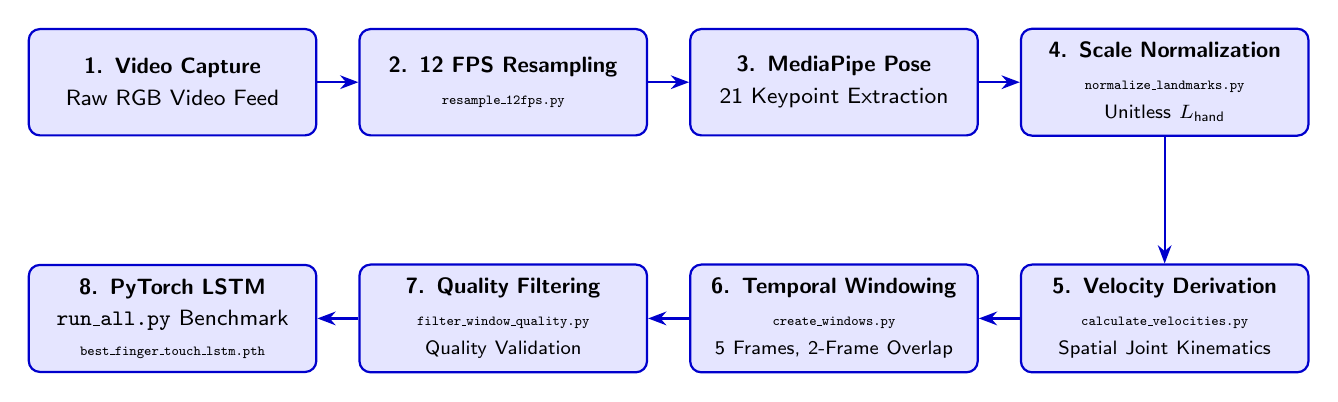
\begin{tikzpicture}[
    block/.style = {rectangle, draw=blue!80!black, fill=blue!10!white, thick, rounded corners=4pt, align=center, font=\sffamily\footnotesize, text width=3.3cm, minimum height=1.35cm, inner sep=5pt},
    arrow/.style = {draw=blue!80!black, ->, >=Stealth, thick}
]

% Row 1: Steps 1 to 4 (Generous 4.2cm column spacing)
\node (step1) [block] at (0, 0) {\textbf{1. Video Capture}\\[2pt]Raw RGB Video Feed};
\node (step2) [block] at (4.2, 0) {\textbf{2. 12 FPS Resampling}\\[2pt]{\tiny\texttt{resample\_12fps.py}}};
\node (step3) [block] at (8.4, 0) {\textbf{3. MediaPipe Pose}\\[2pt]21 Keypoint Extraction};
\node (step4) [block] at (12.6, 0) {\textbf{4. Scale Normalization}\\[2pt]{\tiny\texttt{normalize\_landmarks.py}}\\[1pt]{\scriptsize Unitless $L_{\text{hand}}$}};

% Row 2: Steps 5 to 8 (Generous 3.0cm row spacing, 1.6cm clear gap between boxes)
\node (step5) [block] at (12.6, -3.0) {\textbf{5. Velocity Derivation}\\[2pt]{\tiny\texttt{calculate\_velocities.py}}\\[1pt]{\scriptsize Spatial Joint Kinematics}};
\node (step6) [block] at (8.4, -3.0) {\textbf{6. Temporal Windowing}\\[2pt]{\tiny\texttt{create\_windows.py}}\\[1pt]{\scriptsize 5 Frames, 2-Frame Overlap}};
\node (step7) [block] at (4.2, -3.0) {\textbf{7. Quality Filtering}\\[2pt]{\tiny\texttt{filter\_window\_quality.py}}\\[1pt]{\scriptsize Quality Validation}};
\node (step8) [block] at (0, -3.0) {\textbf{8. PyTorch LSTM}\\[2pt]\texttt{run\_all.py} Benchmark\\[1pt]{\tiny\texttt{best\_finger\_touch\_lstm.pth}}};

% Row 1 Forward Flow
\draw [arrow] (step1.east) -- (step2.west);
\draw [arrow] (step2.east) -- (step3.west);
\draw [arrow] (step3.east) -- (step4.west);

% Transition Down to Row 2 (Clear 1.6cm vertical arrow, zero overlap)
\draw [arrow] (step4.south) -- (step5.north);

% Row 2 Reverse Flow
\draw [arrow] (step5.west) -- (step6.east);
\draw [arrow] (step6.west) -- (step7.east);
\draw [arrow] (step7.west) -- (step8.east);

\end{tikzpicture}

\end{document}
